\usetikzlibrary{shapes}
\usetikzlibrary{decorations.shapes}
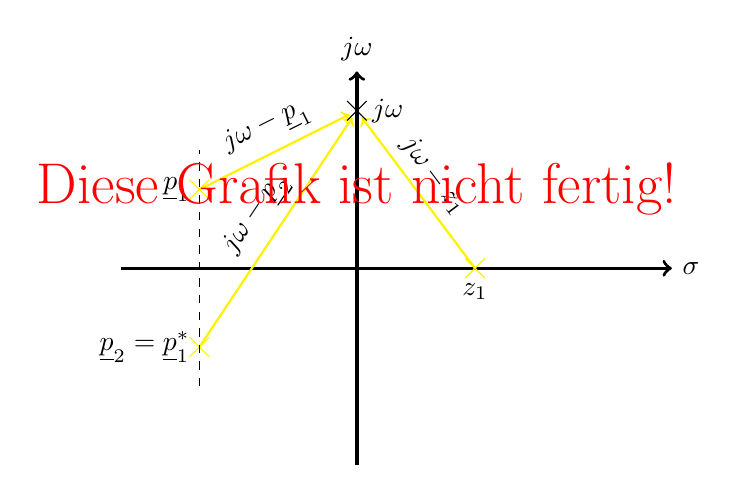
\begin{tikzpicture}

\begin{scope}[->, very thick]
\draw (-3,0) -- (4,0) node[right] {$\sigma$};
\draw (0,-2.5) -- (0,2.5) node[above] {$j\omega$};
\end{scope}

\draw (-2,1) node[cross out, draw=yellow] {} node[left] {$\underline{p}_1$};
\draw (-2,-1) node[cross out, draw=yellow] {} node[left] {$\underline{p}_2 = \underline{p}_1^*$};
\draw (1.5,0) node[cross out, draw=yellow] {} node[below=2] {$z_1$};

\begin{scope}[yellow, ->, thick, shorten >= 3pt]
\draw (-2,1) -- (0,2) node[midway,above, sloped, black] {$j\omega -\underline{p}_1$};
\draw (-2,-1) -- (0,2) node[midway,above, sloped, black] {$j\omega - \underline{p}_2$};;
\draw (1.5,0) -- (0,2) node[midway,above, sloped, black] {$j\omega - z_1$};;
\end{scope}

\draw (0,2) node[cross out, draw] {} node[right=2] {$j\omega$};

\draw[dashed, very thin]  (-2,-1.5) -- +(0,3);

\node[red] at (0,1) {\huge{Diese Grafik ist nicht fertig!}};


\end{tikzpicture}